\documentclass[aps,prb,twocolumn,superscriptaddress,floatfix,longbibliography]{revtex4-2}

\usepackage[utf8]{inputenc}
\usepackage[spanish]{babel}
\usepackage{graphicx}
\usepackage{amsmath}
\usepackage{subcaption}
\usepackage{wrapfig} 
\usepackage[export]{adjustbox}

\usepackage{amsmath,amssymb} % math symbols
\usepackage{bm} % bold math font
\usepackage{graphicx} % for figures
\usepackage{comment} % allows block comments
\usepackage{textcomp} % This package is just to give the text quote '
\usepackage{listings} %para agregar código

%\usepackage{ulem} % allows strikeout text, e.g. \sout{text}

\usepackage[spanish]{babel}

\usepackage{enumitem}
\setlist{noitemsep,leftmargin=*,topsep=0pt,parsep=0pt}

\usepackage{xcolor} % \textcolor{red}{text} will be red for notes
\definecolor{lightgray}{gray}{0.6}
\definecolor{medgray}{gray}{0.4}

\usepackage{hyperref}
\hypersetup{
colorlinks=true,
urlcolor= blue,
citecolor=blue,
linkcolor= blue,
bookmarks=true,
bookmarksopen=false,
}

% Code to add paragraph numbers and titles
\newif\ifptitle
\newif\ifpnumber
\newcounter{para}
\newcommand\ptitle[1]{\par\refstepcounter{para}
{\ifpnumber{\noindent\textcolor{lightgray}{\textbf{\thepara}}\indent}\fi}
{\ifptitle{\textbf{[{#1}]}}\fi}}
%\ptitletrue  % comment this line to hide paragraph titles
%\pnumbertrue  % comment this line to hide paragraph numbers

% minimum font size for figures
\newcommand{\minfont}{6}

% Uncomment this line if you prefer your vectors to appear as bold letters.
% By default they will appear with arrows over them.
% \renewcommand{\vec}[1]{\bm{#1}}

%Cambiar Cuadros por Tablas y lista de...
%\renewcommand{\listtablename}{Índice de tablas}
\renewcommand{\tablename}{Tabla}
\renewcommand{\date}{Fecha}

% \graphicspath{ {C:/Users/lupam/Mi unidad/Pablo Chehade/Instituto Balseiro (IB)/Laboratorio Avanzado/Informe/V5/Figures} } %Para importar imagenes desde una carpeta


\lstset{
  basicstyle=\ttfamily\small,
  breaklines=true,
  frame=single,
  numbers=left,
  numberstyle=\tiny,
  keywordstyle=\color{blue},
  commentstyle=\color{green},
  stringstyle=\color{red},
} %Configuración para el bloque de código


\usepackage[bottom]{footmisc} %para que las notas al pie aparezcan en la misma página



\begin{comment}

%Comandos de interes:

* Para ordenar el documento:
\section{Introducción}
\section{\label{sec:Formatting}Formatting} %label para luego hacer referencia a esa sección

\ptitle{Start writing while you experiment} %pone nombre y título al documento dependiendo de si en el header están los comandos \ptitletrue y \pnumbertrue

* Ecuaciones:
\begin{equation}
a^2+b^2=c^2 \,.
\label{eqn:Pythagoras}
\end{equation}

* Conjunto de ecuaciones:
\begin{eqnarray}
\label{eqn:diagonal}
\nonumber d & = & \sqrt{a^2 + b^2 + c^2} \\
& = & \sqrt{3^2+4^2+12^2} = 13
\end{eqnarray}

* Para hacer items / enumerar:
\begin{enumerate}
  \item
\end{enumerate}

\begin{itemize}
  \item
\end{itemize}

* Figuras:
\begin{figure}[h]
    \includegraphics[clip=true,width=\columnwidth]{pixel-compare}
    \caption{}
     \label{fig:pixels}
\end{figure}

* Conjunto de figuras:
(no recuerdo)


* Para hacer referencias a fórmulas, tablas, secciones, ... dentro del documento:
\ref{tab:spacing}

* Para citar
Elementos de .bib
\cite{WhitesidesAdvMat2004}
url
\url{http://www.mendeley.com/}\\

* Agradecimientos:
\begin{acknowledgments}
We acknowledge advice from Jessie Zhang and Harry Pirie to produce Fig.\ \ref{fig:pixels}.
\end{acknowledgments}

* Apéndice:
\appendix
\section{\label{app:Mendeley}Mendeley}

* Bibliografía:
\bibliography{Hoffman-example-paper}

\end{comment}



\begin{document}

% Allows to rewrite the same title in the supplement
\newcommand{\mytitle}{Aprendizaje supervisado en redes multicapa}

\title{\mytitle}

\author{Pablo Chehade \\
    \small \textit{pablo.chehade@ib.edu.ar} \\
    \small \textit{Redes Neuronales, Instituto Balseiro, CNEA-UNCuyo, Bariloche, Argentina, 2023} \\}
    
\maketitle

\section*{Ejercicio 1}

Se implementaron dos arquitecturas para el aprendizaje de la regla XOR, las cuales se ilustran en la figura \ref{fig:ej1_arquitectura}, considerando, en cada caso, una entrada adicional para simular el bias.

\begin{figure}[h]
    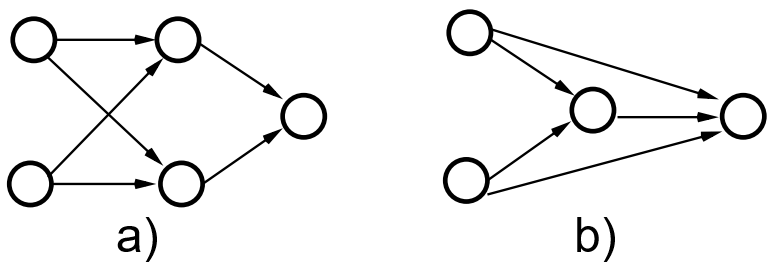
\includegraphics[clip=true,width=\columnwidth]{ej1_arquitectura.png}
    \caption{Arquitecturas utilizadas para el aprendizaje de la regla XOR, denominadas como arquitecturas a) A y b) B.}
     \label{fig:ej1_arquitectura}
\end{figure}

\begin{figure}[h]
    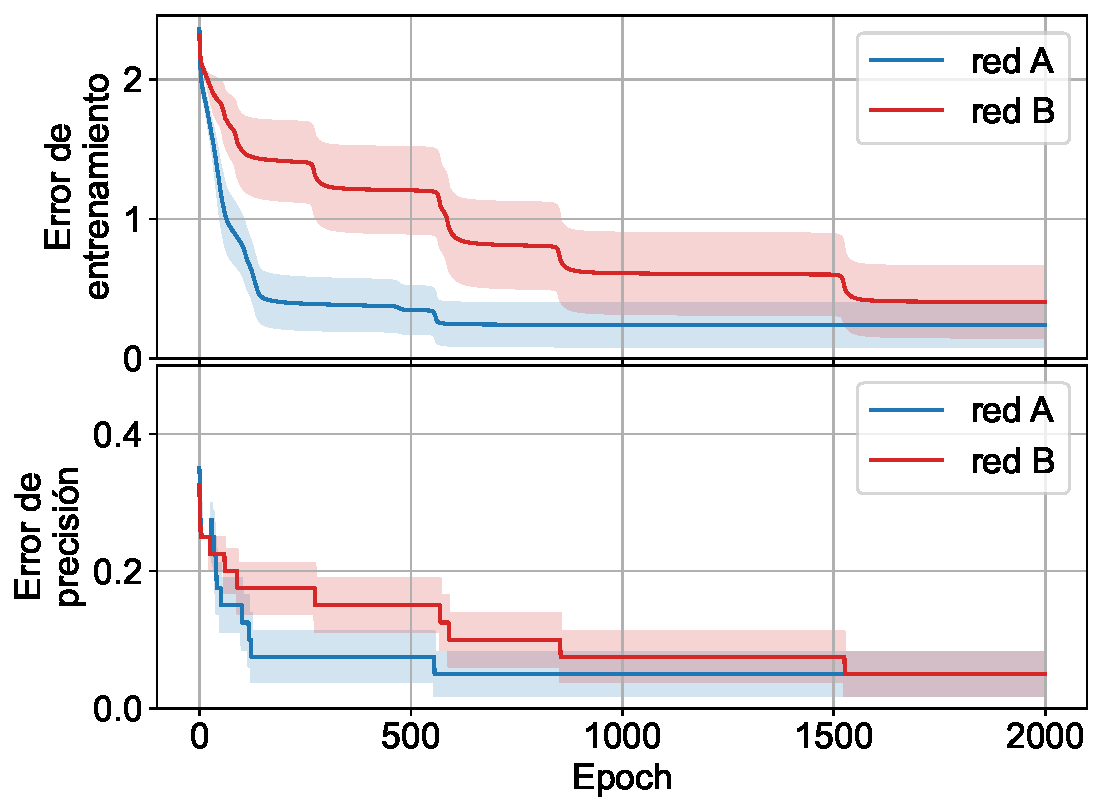
\includegraphics[clip=true,width=\columnwidth]{ej1_vs_epochs.pdf}
    \caption{Valor medio del a) error de entrenamiento y b) error de precisión en función de las epochs de entrenamiento para las arquitecturas A y B. El sombreado indica la desviación estándar del promedio.}
     \label{fig:ej1_error}
\end{figure}

\begin{figure}[h]
    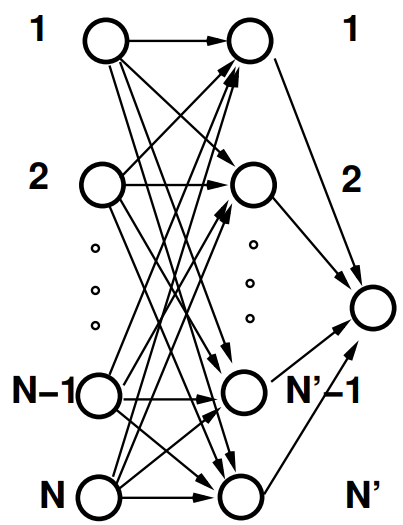
\includegraphics[clip=true,width=0.5\columnwidth]{ej2_arquitectura.png}
    \caption{Arquitectura utilizada para abordar el problema de paridad.}
     \label{fig:ej2_arquitectura}
\end{figure}


\begin{figure}
    {figure}[h]
        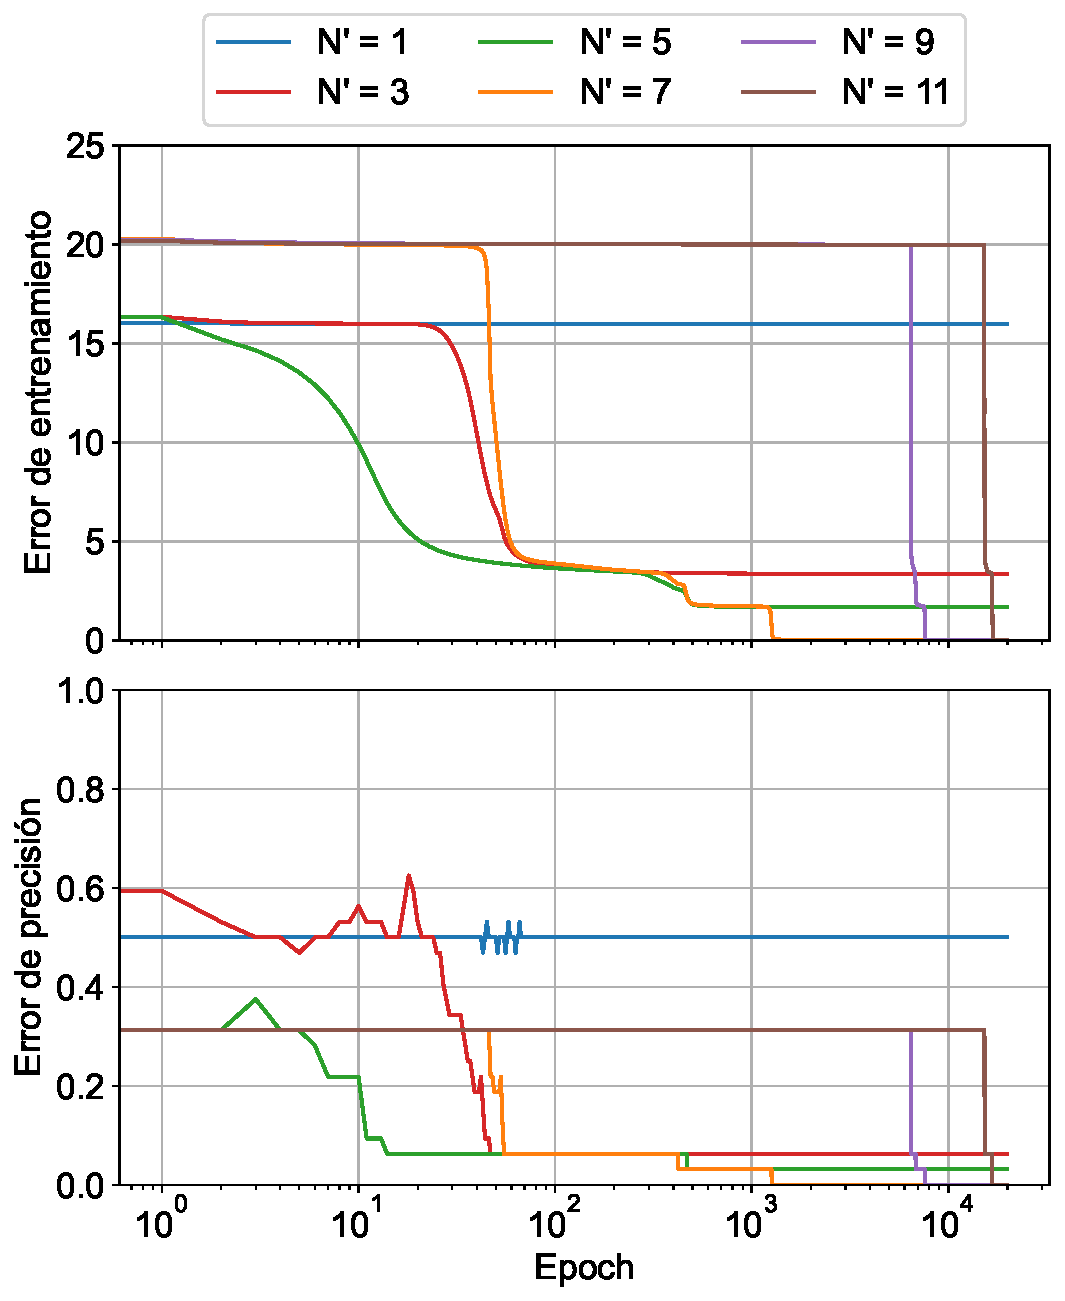
\includegraphics[clip=true,width=\columnwidth]{ej2_vs_epochs.pdf}
        \caption{a) Error de entrenamiento y b) error de precisión en función de las epochs de entrenamiento, variando el número de neuronas N’ en la capa oculta.}
         \label{fig:ej2_error}
\end{figure}
    
    

\begin{figure}[h]
    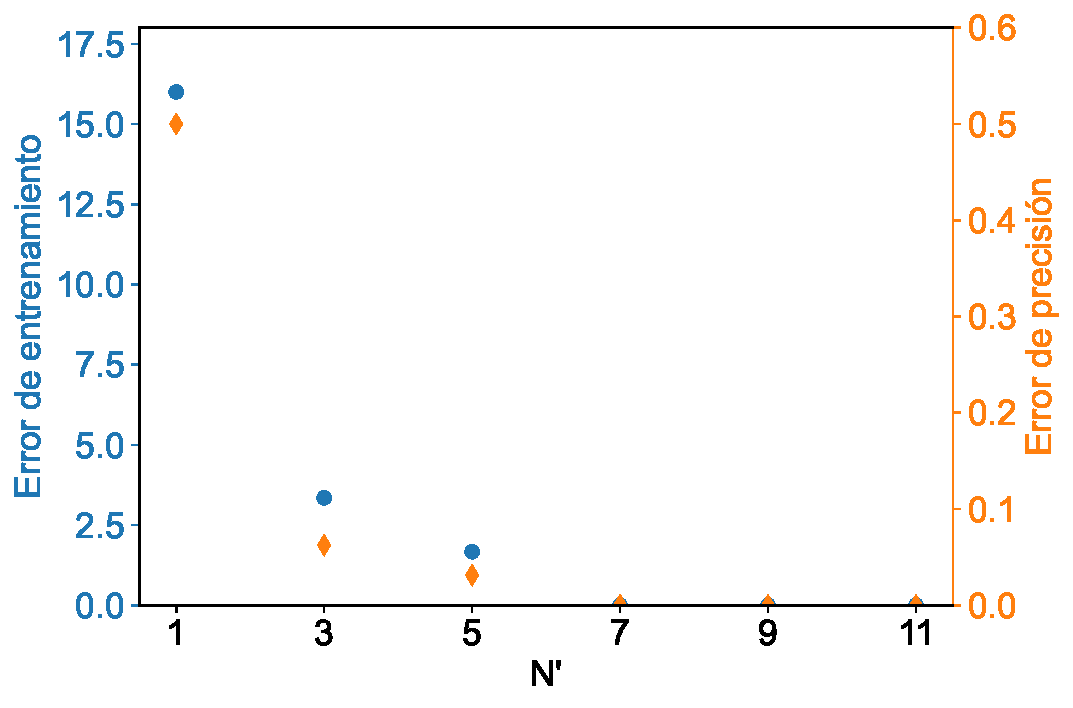
\includegraphics[clip=true,width=\columnwidth]{ej2_vs_N_prima.pdf}
    \caption{Error de entrenamiento y error de precisión final en función del número de neuronas N' en la capa oculta.}
        \label{fig:ej2_error_vs_Nprima}
\end{figure}

\begin{figure}[h]
    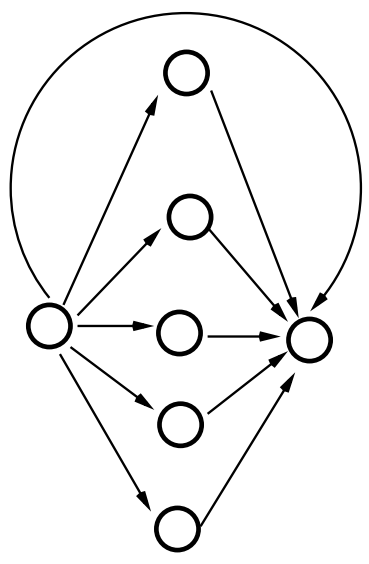
\includegraphics[clip=true,width=0.55\columnwidth]{ej3_arquitectura.png}
    \caption{Arquitectura adoptada para el aprendizaje del mapeo logístico.}
        \label{fig:ej3_arquitectura}
\end{figure}


\begin{figure}[h]
    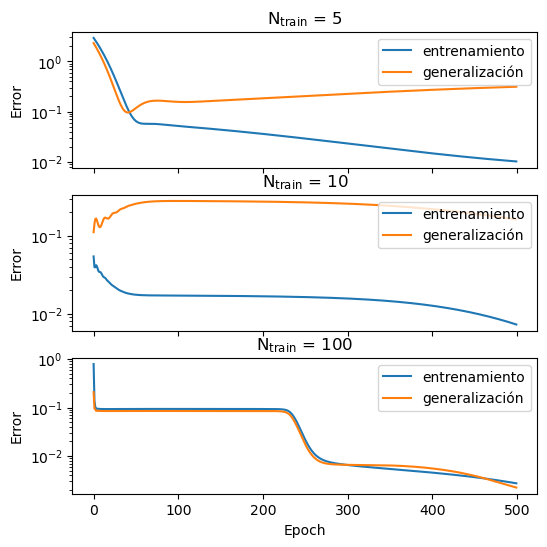
\includegraphics[clip=true,width=\columnwidth]{ej3_vs_epochs.png}
    \caption{Error de entrenamiento y error de generalización en función de las epochs de entrenamiento, para distinto número de ejemplos \(N_{train}\) en los datos de entrenamiento.}
        \label{fig:ej3_error}
\end{figure}


El aprendizaje fue ejecutado mediante el algoritmo de retropropagación de errores (back-propagation), con pesos inicializados aleatoriamente con un valor máximo de 0.1 y un learning rate establecido en 0.1. La función de costo empleada fue el error cuadrático medio (MSE) y se utilizó $f(x) = tanh(x)$ como función de transferencia. Los datos de entrenamiento engloban todas las posibles combinaciones de entradas y salidas. Mientras que los datos de test corresponden al mismo conjunto de datos de entrenamiento.

En la Figura \ref{fig:ej1_error} se grafican los valores medios del error de entrenamiento y de precisión en función de las epochs para ambas arquitecturas, promediados sobre 10 condiciones iniciales de los pesos. En ambas arquitecturas, se evidencia una disminución de los errores a lo largo del tiempo, sin alcanzar un error nulo debido a que algunas redes se estabilizan en mínimos locales. De forma comparativa, la arquitectura A demuestra un tiempo medio de convergencia menor a la B.


Además, se observó cualitativamente que la velocidad de convergencia es influenciada por el valor máximo posible en la inicialización de los pesos y por el learning rate, existiendo configuraciones de ambos parámetros en las cuales el error no converge.

\section*{Ejercicio 2}



Se abordó la resolución del problema de paridad, extendiendo la lógica del XOR a N entradas. La arquitectura utilizada se muestra en la figura \ref{fig:ej2_arquitectura}, habiendo N' neuronas en la capa oculta y añadiendo una entrada adicional para simular el bias. El entrenamiento se llevó a cabo a través del algoritmo de retropropagación de errores, manteniendo la función de transferencia y la inicialización de los pesos idénticas al ejercicio previo y un learning rate de 0.05. Se establecieron N = 5 y N' = 1, 3, 5, 7, 9 y 11. Al igual que antes, los datos de entrenamiento engloban todas las posibles combinaciones de entradas y salidas. Mientras que los datos de test corresponden al mismo conjunto de datos de entrenamiento.


En la figura \ref{fig:ej2_error} se grafica el error de entrenamiento y de precisión en función de las epochs, explorando los diversos valores de N'. Se observa que para N' = 1 el método converge pero con un gran error. Para N' = 3, la convergencia es más gradual hacia un error menor que el anterior pero no nulo. Con incrementos en N', la tendencia persiste: la convergencia es más lenta pero converge hacia errores progresivamente menores. Cuando $\mathrm{N'} > 5$, el error se anula pasado cierto número de epochs. Este fenómeno es evidenciado de forma más clara en la figura \ref{fig:ej2_error_vs_Nprima}, donde se grafica el error final en función de N'. Se observa que el error decae con el aumento de N', directamente relacionado con el aumento de la complejidad de la red.



\section*{Ejercicio 3}

Se procedió al aprendizaje del mapeo logístico utilizando el método de retropropagación de errores, con la arquitectura representada en la figura \ref{fig:ej3_arquitectura} y añadiendo una entrada adicional para simular el bias. Se estableció un learning rate de 0.01 y, para las capas ocultas, se implementó la función de transferencia g(x) = 1/(1 + exp(-x)), mientras que la neurona de salida adoptó una función de activación lineal. Se generaron los \(N_{train}\) datos de entrenamiento a través de la iteración del mapeo \(x(t + 1) = 4x(t)(1-x(t))\). De este modo, los datos corresponden a los pares \{x(t), x(t+1)\}. Además, se utilizaron 100 datos generados de manera análoga como ejemplos de prueba.

En la figura \ref{fig:ej3_error} se grafica el error de entrenamiento y el error de generalización, calculado sobre los datos de prueba, en función de las epochs. Para \(N_{train} = 5\) y 10, el comportamiento observado indica que, ante un número bajo de epochs, se está en condiciones de underfitting; luego, el error de generalización alcanza un mínimo y, posteriormente, aumenta, indicando una condición de overfitting. En cambio, para \(N_{train} = 100\), la gran cantidad de datos permite que ambos errores sean muy similares, sin llegar a presentar overfitting. Este comportamiento con variaciones en \(N_{train}\) se justifica en que el error de generalización tiende a disminuir con la cantidad de ejemplos.



\onecolumngrid

\section*{Apéndice}
A continuación se desarrolla el código empleado durante este trabajo implementado en Python.




\begin{lstlisting}[language=Python]
  #Import libraries
  import numpy as np
  import matplotlib
  import matplotlib.pyplot as plt
  import tensorflow as tf
  
  
  # ### Defino datos
  
  #Def regla XOR
  def XOR(x1, x2):
      #x1, x2: +1 o -1
      if x1 == x2:
          return 1
      else:
          return -1
  
  #Def datos x e y
  x_data = np.empty([4, 2])
  y_data = np.empty(4)
  x_data[0] = np.array([1,1])
  x_data[1] = np.array([1,-1])
  x_data[2] = np.array([-1,1])
  x_data[3] = np.array([-1,-1])
  for i in range(len(y_data)):
      y_data[i] = XOR(x_data[i][0], x_data[i][1])
  
  # ### Defino funciones
  
  #Def la aplicación de una red
  def red_forward(x_test, red):
      V_0 = np.concatenate((x_test, np.array([-1])), axis = 0) #Agrego el bias 3x1
      for j in range(len(red["pesos"])):
          w = red["pesos"][j]
          h = np.dot(w.T, V_0)
          if j != len(red["pesos"]) - 1:
              V_1 = np.concatenate((g(h), np.array([-1])), axis = 0) #3x1
          else: #Si estoy en la última capa
              V_1 = g(h)
          V_0 = V_1
      return V_1[0]
  
  #Def función de validación
  def validacion(x_test, y_test, red):
      error = 0
      for i in range(len(y_test)):
          #Forward pass
          y_out = red_forward(x_test[i], red)
          #Aproximo y_out para que sea +1 o -1
          if y_out >= 0:
              y_out = 1
          else:
              y_out = -1
          #Calculo el error
          error += np.abs(y_test[i] - np.round(y_out))/2 #Da 0 si no hay error y 1 si hay error
      return error/len(y_test)
  
  def e_loss(x_test, y_test, red):
      error = 0
      for i in range(len(y_test)):
          #Forward pass
          y_out = red_forward(x_test[i], red)
          #Calculo el error
          error += (y_test[i] - y_out)**2
      return error/2
  
  #Def función de transferencia
  def g(h_vec):
      return np.tanh(h_vec)
  
  def g_prima(h_vec):
      return 1 - g(h_vec)**2
  
  
  #Def algoritmo de retropropagación de errores
  def back_propagation(x_data, y_data, red, eta):
      #Se usa la nomenclatura del Hertz
      #Loop sobre las muestras
      for i in range(len(y_data)):   
          #Forward pass
          V_0 = np.concatenate((x_data[i], np.array([-1])), axis = 0) #Agrego el bias 3x1
          w_1 = red["pesos"][0] #3x2
          h_1 = np.dot(w_1.T, V_0) #2x1
          V_1 = np.concatenate((g(h_1), np.array([-1])), axis = 0) #3x1
          w_2 = red["pesos"][1] #3x1
          h_2 = np.dot(w_2.T, V_1) #1x1
          V_2 = g(h_2) #1x1
          #Backward
          #Calculo el error de la capa de salida
          delta_2 = g_prima(h_2)*(y_data[i] - V_2) #1x1
          #Calculo el error de la capa oculta
          # delta_1 = g_prima(h_1)*np.dot(w_2, delta_2) #
          delta_1 = np.concatenate([g_prima(h_1),np.array([1])])*np.dot(w_2, delta_2) #3x1
          #Actualizo pesos
          w_1 += eta * np.outer(V_0, delta_1[:-1]) #3x2
          w_2 += eta * np.outer(V_1, delta_2)
          if red["name"] == "B":
              #Tengo que fijar algunos elementos de los pesos para que no varíen
              w_1[0,0] = 1; w_1[0,2] = 0
              w_1[1,0] = 0; w_1[1,2] = 1
              w_1[2,0] = 0; w_1[2,2] = 0
          red["pesos"] = [w_1, w_2]
      return red
  
  #Def algoritmo de aprendizaje
  def aprendizaje(x_data, y_data, red, eta, epochs = 1):
      #Def array de errores
      e_loss_vec = np.empty(epochs)
      validacion_vec = np.empty(epochs)
      #Loop sobre las epochs
      for i in range(epochs):
          #Backpropagation
          red = back_propagation(x_data, y_data, red, eta)
          #Cálculo de errores
          e_loss_vec[i] = e_loss(x_data, y_data, red)
          validacion_vec[i] = validacion(x_data, y_data, red)
      return red, e_loss_vec, validacion_vec
  
  # ### Aprendizaje
  # 
  # Para cada arquitectura repito el entrenamiento con 10 condiciones iniciales distintas
  
  np.random.seed(1) #def seed
  N_CI = 10 #Nro de condiciones iniciales
  N_epochs = 2000 #nro de epochs que voy a entrenar
  
  def red_A(w_ini_max):
      #Cambia en cada llamada por los nros random
      return {"name": "A", "input":2, "hidden":2, "output":1, "pesos":[np.random.rand(3,2)*w_ini_max, np.random.rand(3,1)*w_ini_max]}
  def red_B(w_ini_max):
      #Para modelar la neurona B, agrego en la capa oculta 2 neuronas que van a ser una copia directa de las neuronas previas correspondientes. Esto tengo que modificarlo a mano luego
      return {"name": "B" , "input":2, "hidden":2, "output":1, "pesos":[np.random.rand(3,3)*w_ini_max, np.random.rand(4,1)*w_ini_max]}
  
  def aprendizaje_redes(N_CI, N_epochs, red, x_data, y_data, eta = 0.1):
      #red escrita como función, de modo de que cambie los pesos en cada CI
      w_ini_max = 1 #peso máximo en la inicialización
      e_loss_matrix = np.empty([N_CI, N_epochs])
      validation_matrix = np.empty([N_CI, N_epochs])
      for i in range(N_CI):
          #Entreno red
          model_A = aprendizaje(x_data, y_data, red(w_ini_max), eta, epochs = N_epochs)
          #Guardo el error
          e_loss_matrix[i] = model_A[1]
          validation_matrix[i] = model_A[2]
      #Calculo media y desviación estándar de la media de los errores a cada tiempo
      e_loss_mean = np.mean(e_loss_matrix, axis = 0)
      e_loss_std = np.std(e_loss_matrix, axis = 0)/np.sqrt(N_CI)
      validation_mean = np.mean(validation_matrix, axis = 0)
      validation_std = np.std(validation_matrix, axis = 0)/np.sqrt(N_CI)
      red_final = model_A[0]
      return e_loss_mean, e_loss_std, validation_mean, validation_std, red_final
  
  A_e_loss_mean, A_e_loss_std, A_validation_mean, A_validation_std, A_red_final = aprendizaje_redes(N_CI, N_epochs, red_A, x_data, y_data)
  B_e_loss_mean, B_e_loss_std, B_validation_mean, B_validation_std, B_red_final = aprendizaje_redes(N_CI, N_epochs, red_B, x_data, y_data)
  
  #Grafico
  
  fig, ax = plt.subplots(2, 1, figsize = (8,6), sharex=True)
  fig.subplots_adjust(hspace=0.02)
  
  #Red A:
  ax[0].plot(A_e_loss_mean, label = "red A", color = "tab:blue")
  ax[0].fill_between(np.arange(N_epochs), A_e_loss_mean - A_e_loss_std, A_e_loss_mean + A_e_loss_std, alpha = 0.2, color = "tab:blue")
  ax[1].plot(A_validation_mean, label = "red A", color = "tab:blue")
  ax[1].fill_between(np.arange(N_epochs), A_validation_mean - A_validation_std, A_validation_mean + A_validation_std, alpha = 0.2, color = "tab:blue")
  #Red B:
  ax[0].plot(B_e_loss_mean, label = "red B", color = "tab:red")
  ax[0].fill_between(np.arange(N_epochs), B_e_loss_mean - B_e_loss_std, B_e_loss_mean + B_e_loss_std, alpha = 0.2, color = "tab:red")
  ax[1].plot(B_validation_mean, label = "red B", color = "tab:red")
  ax[1].fill_between(np.arange(N_epochs), B_validation_mean - B_validation_std, B_validation_mean + B_validation_std, alpha = 0.2, color = "tab:red")
  
  #Decoración
  ax[1].set_xlabel("Epoch")
  ax[0].set_ylabel("Error de\nentrenamiento")
  ax[1].set_ylabel("Error de\nprecisión")
  ax[0].grid(); ax[1].grid()
  ax[0].set_ylim([0, np.max(np.array([np.max(A_e_loss_mean + A_e_loss_std), np.max(B_e_loss_mean + B_e_loss_std)] ) )])
  ax[1].set_ylim([0, 0.5])
  ax[0].legend()
  ax[1].legend()
  plt.show()
  
  # ## Ejercicio 2
  from itertools import product
  
  #Defino ejemplos a aprender
  def XOR_gral(x_vec):
      #x[i] = +/- 1 for all i
      return np.prod(x_vec, axis = 0) 
  
  def generate_matrix(N):
      # Generar todas las combinaciones posibles de 0s y 1s de longitud N
      combinations = product([-1, 1], repeat=N)
      # Convertir las combinaciones a una matriz de numpy
      matrix = np.array(list(combinations))
      return matrix
  
  def RN_XOR_gral(N_prima_array, x_data, y_data, N_CI, N_epochs, eta = 0.1):
      N = len(x_data[0]) #Nro de entradas
      #Def la seed
      np.random.seed(1) #Para obtener siempre el mismo resultado
      e_loss_mean_matrix = np.empty([len(N_prima_array), N_epochs])
      e_loss_std_matrix = np.empty([len(N_prima_array), N_epochs])
      validation_mean_matrix = np.empty([len(N_prima_array), N_epochs])
      validation_std_matrix = np.empty([len(N_prima_array), N_epochs])
      for i, N_prima in enumerate(N_prima_array):
          def red_C(w_ini_max):
              return {"name": "C", "input":N, "hidden":N_prima, "output":1, "pesos":[np.random.rand(N+1,N_prima)*w_ini_max, np.random.rand(N_prima+1,1)*w_ini_max]}
          e_loss_mean_matrix[i], e_loss_std_matrix[i], validation_mean_matrix[i], validation_std_matrix[i], red_final = aprendizaje_redes(N_CI, N_epochs, red_C, x_data, y_data, eta = eta)
      return e_loss_mean_matrix, e_loss_std_matrix, validation_mean_matrix, validation_std_matrix
  
  #Genero datos
  
  N = 5
  x_data = generate_matrix(N)
  y_data = np.empty(2**N)
  for i in range(2**N):
      y_data[i] = XOR_gral(x_data[i])
  
  #Entreno
  
  N_prima_array = [1, 3, 5, 7, 9, 11]
  N_CI = 1
  N_epochs = 2*10000
  eta = 0.05 #0.01
  e_loss_mean_matrix, e_loss_std_matrix, validation_mean_matrix, validation_std_matrix = RN_XOR_gral(N_prima_array, x_data, y_data, N_CI, N_epochs, eta)
  
  #Calculo y grafico
  fig, ax = plt.subplots(2, 1, figsize = (8,9), sharex=True, squeeze=True)
  #Junto las subplots 
  fig.subplots_adjust(hspace=0.1)
  
  #labels
  N_prima_labels = []
  for i in range(len(N_prima_array)):
      N_prima_labels.append("N' = " + str(N_prima_array[i]))
  colors = ["tab:blue", "tab:red", "tab:green", "tab:orange", "tab:purple", "tab:brown"]
  #Grafico e_loss_mean_matrix.T
  for i in range(len(N_prima_array)):
      ax[0].plot(e_loss_mean_matrix[i], label = N_prima_labels[i], color = colors[i])
      ax[0].fill_between(np.arange(N_epochs), e_loss_mean_matrix[i] - e_loss_std_matrix[i], e_loss_mean_matrix[i] + e_loss_std_matrix[i], alpha = 0.2)
  for i in range(len(N_prima_array)):
      ax[1].plot(validation_mean_matrix[i], label = N_prima_labels[i], color = colors[i])
      ax[1].fill_between(np.arange(N_epochs), validation_mean_matrix[i] - validation_std_matrix[i], validation_mean_matrix[i] + validation_std_matrix[i], alpha = 0.2)
  
  #Decoración
  ax[1].set_xlabel("Epoch")
  ax[0].set_ylabel("Error de entrenamiento")
  ax[1].set_ylabel("Error de precisión")
  ax[0].set_xscale("log")
  ax[1].set_xscale("log")
  ax[0].set_ylim([0, 25])
  ax[1].set_ylim([0, 1])
  # ax[0].set_ylim([0, np.max(np.array([np.max(A_e_loss_mean + A_e_loss_std), np.max(B_e_loss_mean + B_e_loss_std)] ) )])
  ax[0].grid()
  ax[1].grid()
  #Agrego legend fuera del gráfico arriba de todo
  ax[0].legend(loc = "upper center", bbox_to_anchor=(0.5, 1.3), ncol = 3)
  plt.show()
  
  #Grafico el último valor de error de entrenamiento y de validación como función de N'
  fig, ax = plt.subplots(figsize = (7,5))
  ax.plot(N_prima_array, e_loss_mean_matrix[:,-1], "o")
  ax.set_xlabel("N'")
  ax.set_ylabel("Error de entrenamiento", color = "tab:blue")
  #Agrego los ticks en x sobre N_prima_array
  ax.spines['right'].set_color('tab:blue')
  ax.tick_params(axis='y', colors='tab:blue')
  ax.set_xticks(N_prima_array)
  ax.set_ylim([0,18])
  #En el eje derecho grafico e_validation
  ax2 = ax.twinx()
  #Pinto eje y ticks de naranja
  ax2.spines['right'].set_color('tab:orange')
  ax2.tick_params(axis='y', colors='tab:orange')
  ax2.plot(N_prima_array, validation_mean_matrix[:,-1], "d", color = "tab:orange")
  ax2.set_ylabel("Error de precisión", color = "tab:orange")
  ax2.set_ylim([0, 0.6])
  
  plt.show()
  
  
  # ## Ejercicio 3
  
  #Fijo seed for reproducibility 
  seed=2
  np.random.seed(seed)
  tf.random.set_seed(seed)
  # Data Input
  def mapeo_logistico(x):
      return 4*x*(1-x)
  
  N_train = 100
  N_test = 100
  
  x_train = np.random.rand(N_train)
  x_test = np.random.rand(N_test)
  
  y_train = mapeo_logistico(x_train)
  y_test = mapeo_logistico(x_test)
  
  #Def red
  def output_activation(x):
      return 1/(1 + tf.math.exp(-x))
  
  def RN(x_train, y_train, x_test, y_test, N_epochs = 500):
      # Network architecture
      hidden_dim=5 # Number of hidden units
      inputs = tf.keras.layers.Input(shape=(1,))
      x = tf.keras.layers.Dense(hidden_dim, activation=output_activation)(inputs)
      merge=tf.keras.layers.concatenate([inputs,x],axis=-1)
      predictions = tf.keras.layers.Dense(1)(merge) #si no se declara activation, se usa activation lineal
  
      # Model 
      opti=tf.keras.optimizers.Adam(lr=0.01, decay=0.0)
      model = tf.keras.Model(inputs=inputs, outputs=predictions)
      model.compile(optimizer=opti,
                  loss='MSE') #, metrics=[v1_accuracy]
      history=model.fit(x=x_train, y=y_train,
                      epochs=N_epochs,
                      batch_size=5,
                      shuffle=False,
                      validation_data=(x_test, y_test), verbose=True)
      e_loss = history.history['loss']
      e_validation = history.history['val_loss']
      return e_loss, e_validation
  
  #Varío la cantidad de datos de train
  N_train_vec = [5, 10, 100] #[5,10,20,40,60,80,100]
  N_epochs = 500
  e_loss_matrix = np.empty([len(N_train_vec), N_epochs])
  e_validation_matrix = np.empty([len(N_train_vec), N_epochs])
  for i, N_train in enumerate(N_train_vec):
      e_loss_matrix[i], e_validation_matrix[i] = RN(x_train[:N_train], y_train[:N_train], x_test, y_test, N_epochs)
  
  #Graph
  fig, ax = plt.subplots(len(N_train_vec), 1, figsize = (6,6), sharex = True)
  fig.subplots_adjust(hspace=0.2)
  for i in range(len(N_train_vec)):
      ax[i].plot(e_loss_matrix[i], label='entrenamiento')
      ax[i].plot(e_validation_matrix[i], label='generalización')
      ax[i].set_title("$\mathrm{N_{train}}$ = " + str(N_train_vec[i]))
      # ax[i].set_ylim([0,1.3])
      ax[i].legend(loc = 'upper right')
      ax[i].set_ylabel('Error')
      ax[i].set_yscale("log")
  ax[2].set_xlabel('Epoch')
  plt.show()

\end{lstlisting}

\bibliography{Chehade_practica_4.bib}

\end{document}





